\section*{Aufgabe 8.2}
In dieser Aufgabe sollte die Dichte in Abhängigkeit der Dichte für verschieden Gittergrößen
geplottet werden. Der Code dafür ist bereits in \lref{bond_perk} dargestellt. Die
resultierenden Kurven sind in \fref{dichte} dargestellt.

\begin{figure}[htb]
  \centering
  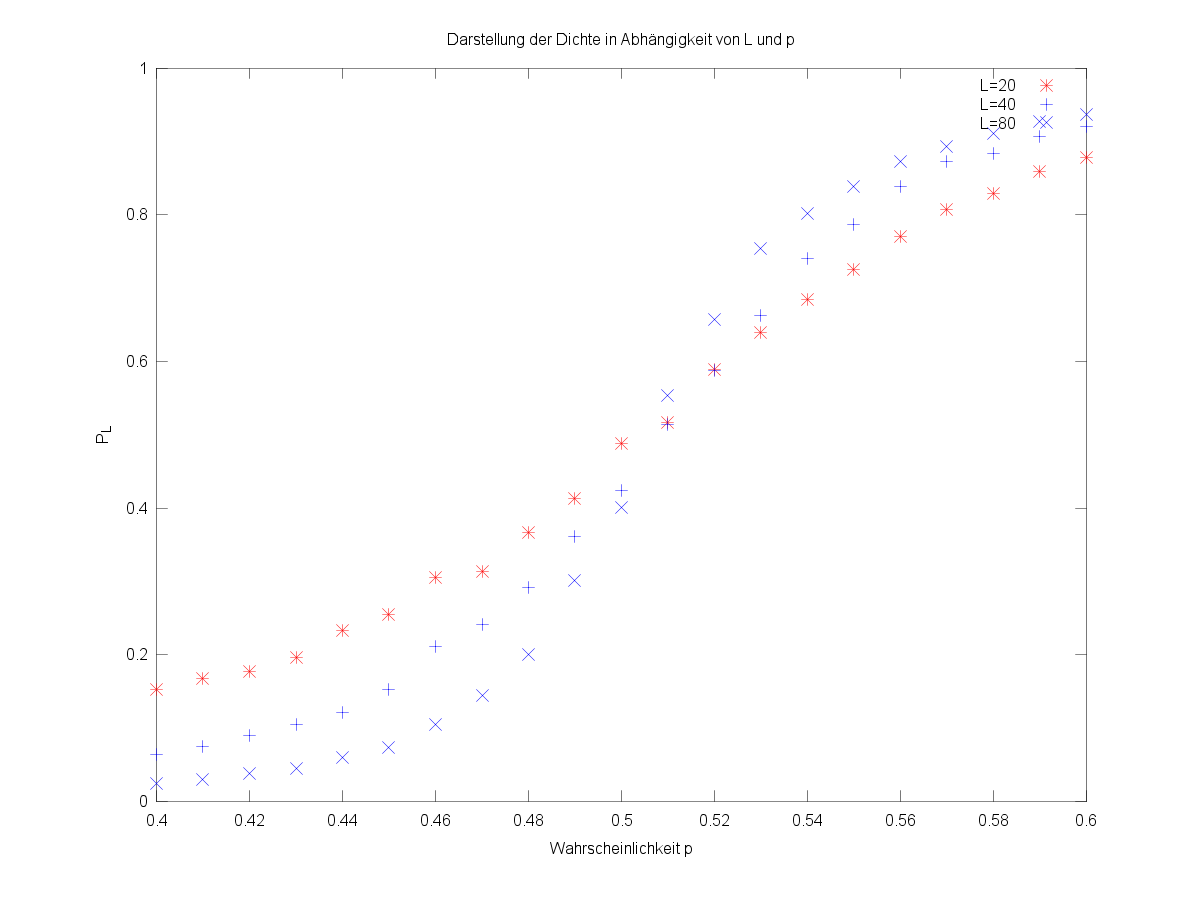
\includegraphics[width=0.8\columnwidth,keepaspectratio]{../tmp/zweitens.png}
  \caption{Dichte in Abhängigkeit von der Wahrscheinlichkeit und für verschiedene Gittergrößen}
  \label{fig:dichte}
\end{figure}